%----------------------------------------------------------------------------------------
%    PACKAGES AND THEMES
%----------------------------------------------------------------------------------------
\documentclass[aspectratio=169,xcolor=dvipsnames]{beamer}
\makeatletter
\def\input@path{{theme/}}
\makeatother
\usetheme{CleanEasy}
\usepackage{lmodern}
\usepackage[T1]{fontenc}
\usepackage[portuguese]{babel}
\usepackage{fix-cm}
\usepackage{amsmath}
\usepackage{mathtools}
\usepackage{listings}
\usepackage{xcolor}
\usepackage{hyperref}
\usepackage{graphicx} % Allows including images
\usepackage{booktabs} % Allows the use of \toprule, \midrule and \bottomrule in tables
\usepackage{tikz}
\usetikzlibrary{positioning, shapes, arrows, calc, decorations.pathreplacing, arrows.meta, backgrounds, patterns, overlay-beamer-styles}
\usepackage{etoolbox}
\usepackage{animate}

%----------------------------------------------------------------------------------------
%    LAYOUT CONFIGURATION
%----------------------------------------------------------------------------------------



% Configure code listings
\lstset{
  basicstyle=\ttfamily\small,
  keywordstyle=\color{blue},
  commentstyle=\color{green!60!black},
  stringstyle=\color{red},
  showstringspaces=false,
  breaklines=true,
  frame=single,
  rulecolor=\color{black!30},
  backgroundcolor=\color{black!5},
  numbers=left,
  numberstyle=\tiny\color{black!70},
  numbersep=5pt
}

%----------------------------------------------------------------------------------------
%    TITLE PAGE
%----------------------------------------------------------------------------------------
%---------------------------------------------


\title[BattAIHealth]{BattAIHealth: AI for Battery Health Monitoring}

\author[Pedro Ferreira]{Pedro André Silva Ferreira}

\institute{Engenharia Eletrotécnica e de Computadores\\Ramo de Eletrónica e Computadores }

\date{21 Julho 2025}
% Define positions for logos on title page
\titlegraphic{
  \begin{tikzpicture}[remember picture, overlay]
    % ESTG Logo
    \node[anchor=north east, xshift=-0.8cm, yshift=-0.3cm] at (current page.north east) {
      
\includegraphics[height=1.5cm]{logos/estg_h.pdf}
    };
  \end{tikzpicture}
}


%----------------------------------------------------------------------------------------

\begin{document}

\begin{frame}[plain]
  \titlepage
\end{frame}

\begin{frame}[plain]{Conteúdos}
  \tableofcontents
\end{frame}

\section{Introdução}
\begin{frame}{Motivação}
  \begin{block}{Contexto}
    \begin{itemize}
      \item Veículos elétricos e comboios eletrificados dependem de monitorização precisa da saúde das baterias
      \item Parâmetros críticos: Estado de carga (SOC), Estado de saúde (SOH) e Vida útil restante (RUL)
      \item Processos químicos complexos que mudam com temperatura, padrões de uso e envelhecimento
    \end{itemize}
  \end{block}
  
  \begin{alertblock}{Limitações dos Métodos Atuais}
    \begin{itemize}
      \item Métodos tradicionais (coulomb counting, filtros de Kalman) têm limitações
      \item Funcionam bem em ambientes controlados, mas falham em condições reais
      \item Acumulação de erros ao longo do tempo
    \end{itemize}
  \end{alertblock}
\end{frame}

\begin{frame}{Objetivos do Trabalho}
  \begin{block}{Objetivo Principal}
    Desenvolver métodos baseados em IA para prever SOC, SOH e RUL simultaneamente e com precisão
  \end{block}
  
  \vspace{0.3cm}
  
  \begin{block}{Parâmetros a Estimar}
    \begin{itemize}
      \item \textbf{Estado de Carga (SOC)}: Energia remanescente na bateria
      \item \textbf{Estado de Saúde (SOH)}: Capacidade atual vs. capacidade original
      \item \textbf{Vida Útil Remanescente (RUL)}: Ciclos até degradação crítica
    \end{itemize}
  \end{block}
  
  \begin{exampleblock}{Contribuições}
    \begin{itemize}
      \item Comparação entre abordagens baseadas em diferentes redes neurais
      \item Adaptação da arquitetura TimesNet para dados de baterias
    \end{itemize}
  \end{exampleblock}
\end{frame}

\section{Fundamentos Teóricos}
\begin{frame}{Conceitos Fundamentais - Parâmetros das Baterias}
  \begin{block}{Estado de Carga (SOC)}
    $$SOC = \frac{\text{Carga Remanescente}}{\text{Capacidade Máxima}} \times 100\%$$
    \begin{itemize}
      \item Estimativa aproximada devido à complexidade química
      \item Não-linearidade causada por degradação dos eletrodos
    \end{itemize}
  \end{block}
  
  \begin{block}{Estado de Saúde (SOH)}
    $$SOH = \frac{\text{Capacidade Máxima Atual}}{\text{Capacidade Máxima Original}} \times 100\%$$
    \begin{itemize}
      \item Fadiga progressiva dos materiais
      \item Diminuição da área superficial ativa
    \end{itemize}
  \end{block}
\end{frame}

\begin{frame}{Visualização da Degradação}
  \begin{columns}[T]
    \begin{column}{0.33\textwidth}
      \centering
      \begin{figure}
        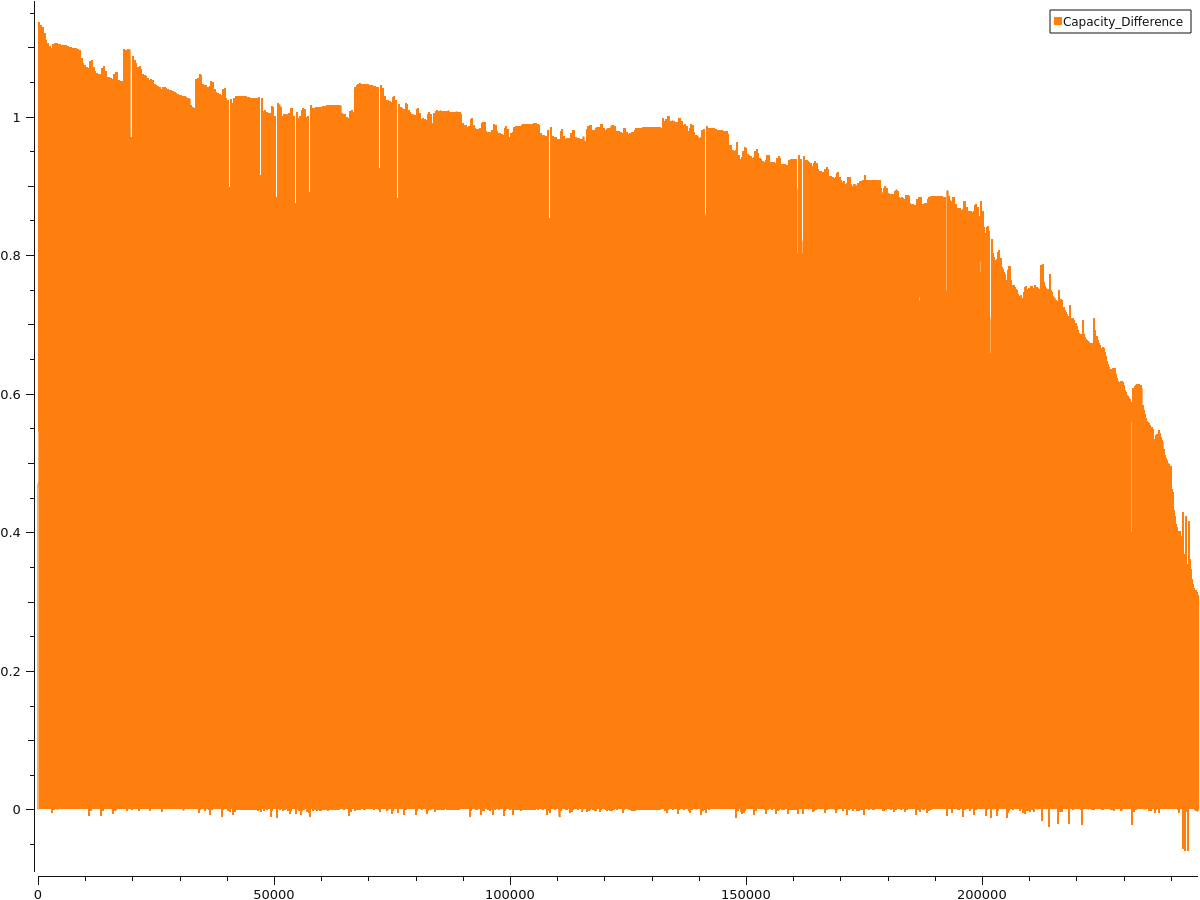
\includegraphics[width=\textwidth]{logos/capacity.png}
        \caption{Capacidade}
      \end{figure}
    \end{column}
    \begin{column}{0.33\textwidth}
      \centering
      \begin{figure}
        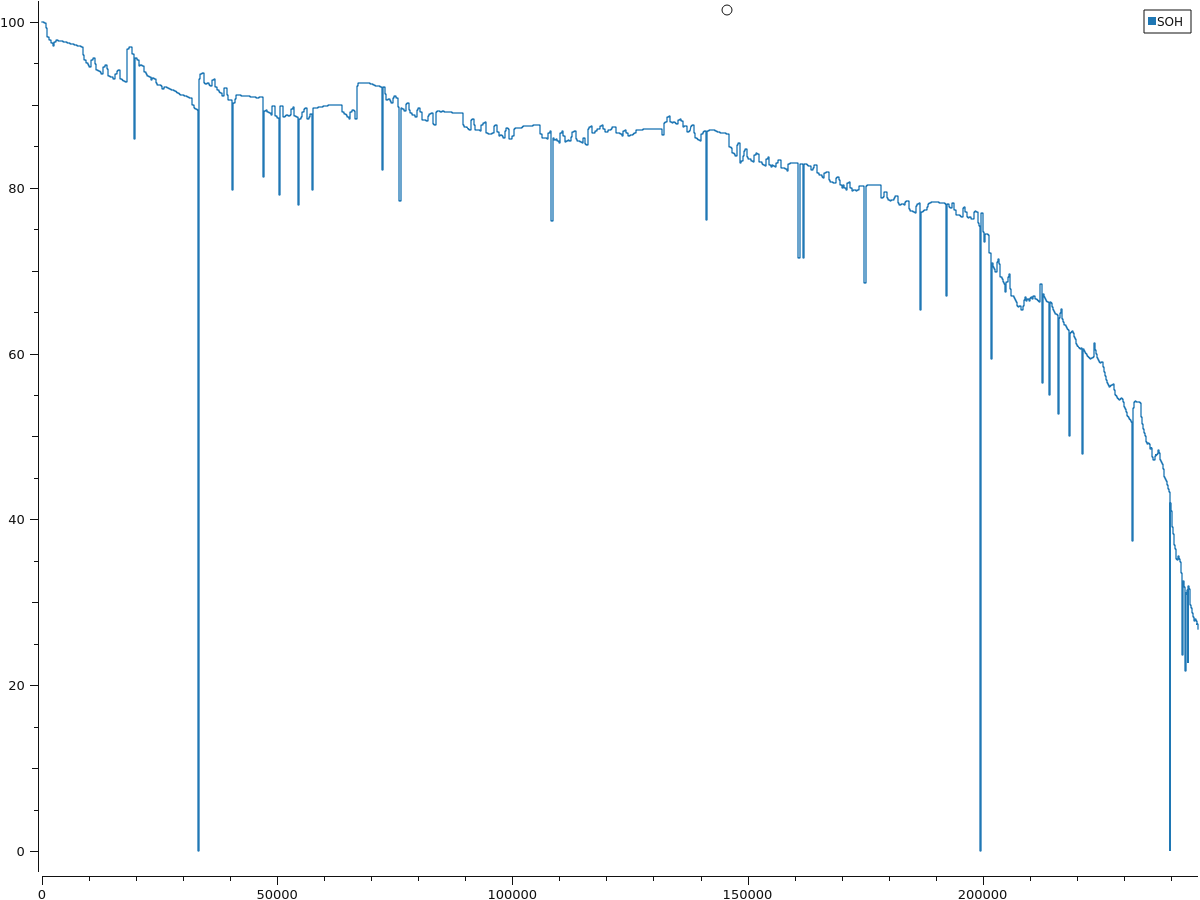
\includegraphics[width=\textwidth]{logos/SOH.png}
        \caption{Estado de Saúde (SOH)}
      \end{figure}
    \end{column}
    \begin{column}{0.33\textwidth}
      \centering
      \begin{figure}
        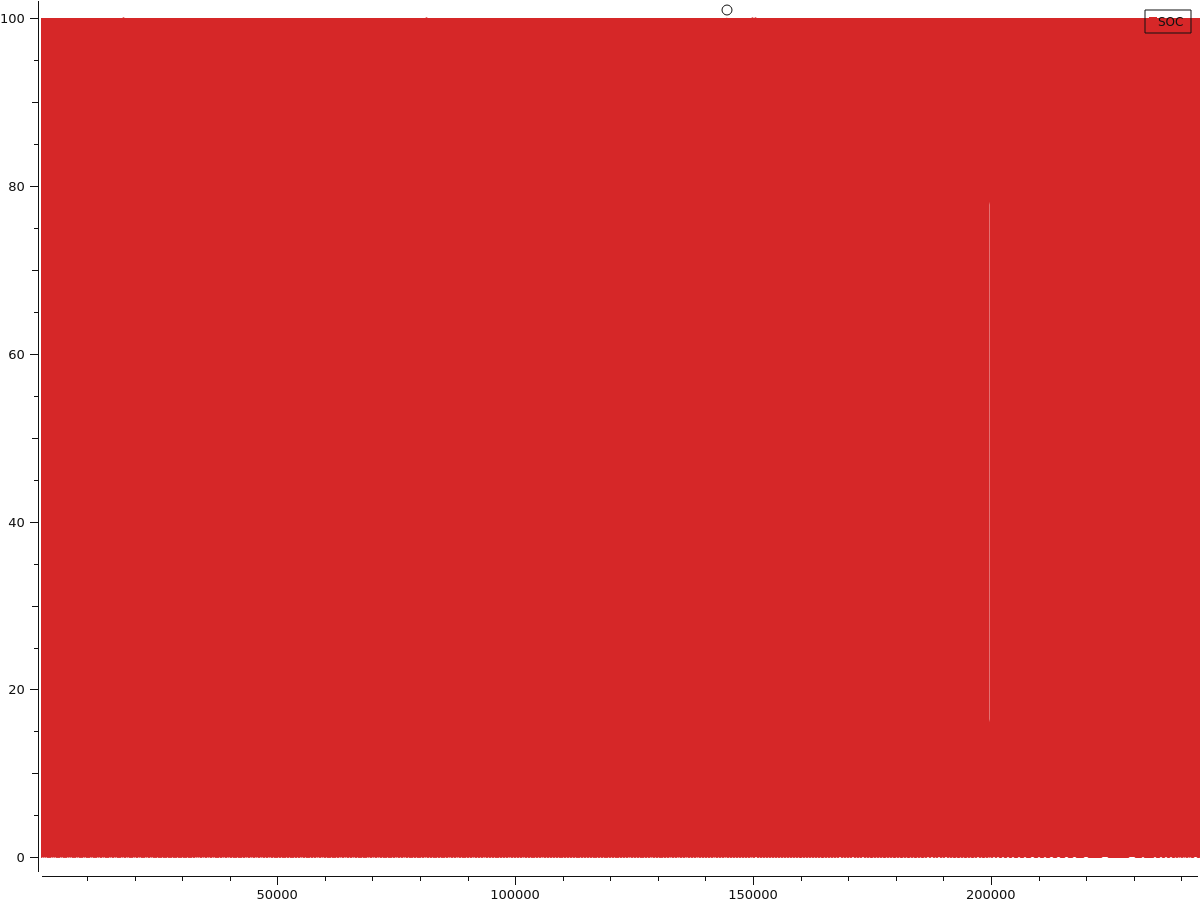
\includegraphics[width=\textwidth]{logos/SOC.png}
        \caption{Estado de Carga (SOC)}
      \end{figure}
    \end{column}
  \end{columns}
\end{frame}

\begin{frame}{Degradação e Envelhecimento das Baterias}
  \begin{columns}[T]
    \begin{column}{0.5\textwidth}
      \begin{alertblock}{Mecanismos de Degradação}
        \begin{itemize}
          \item \textbf{Formação SEI}: Crescimento da interface sólido-eletrólito
          \item \textbf{Perda de Lítio}: Redução do lítio ativo disponível
          \item \textbf{Degradação estrutural}: Mudanças na estrutura dos eletrodos
          \item \textbf{Impedância}: Aumento da resistência interna
        \end{itemize}
      \end{alertblock}
    \end{column}
    \begin{column}{0.5\textwidth}
      \centering
      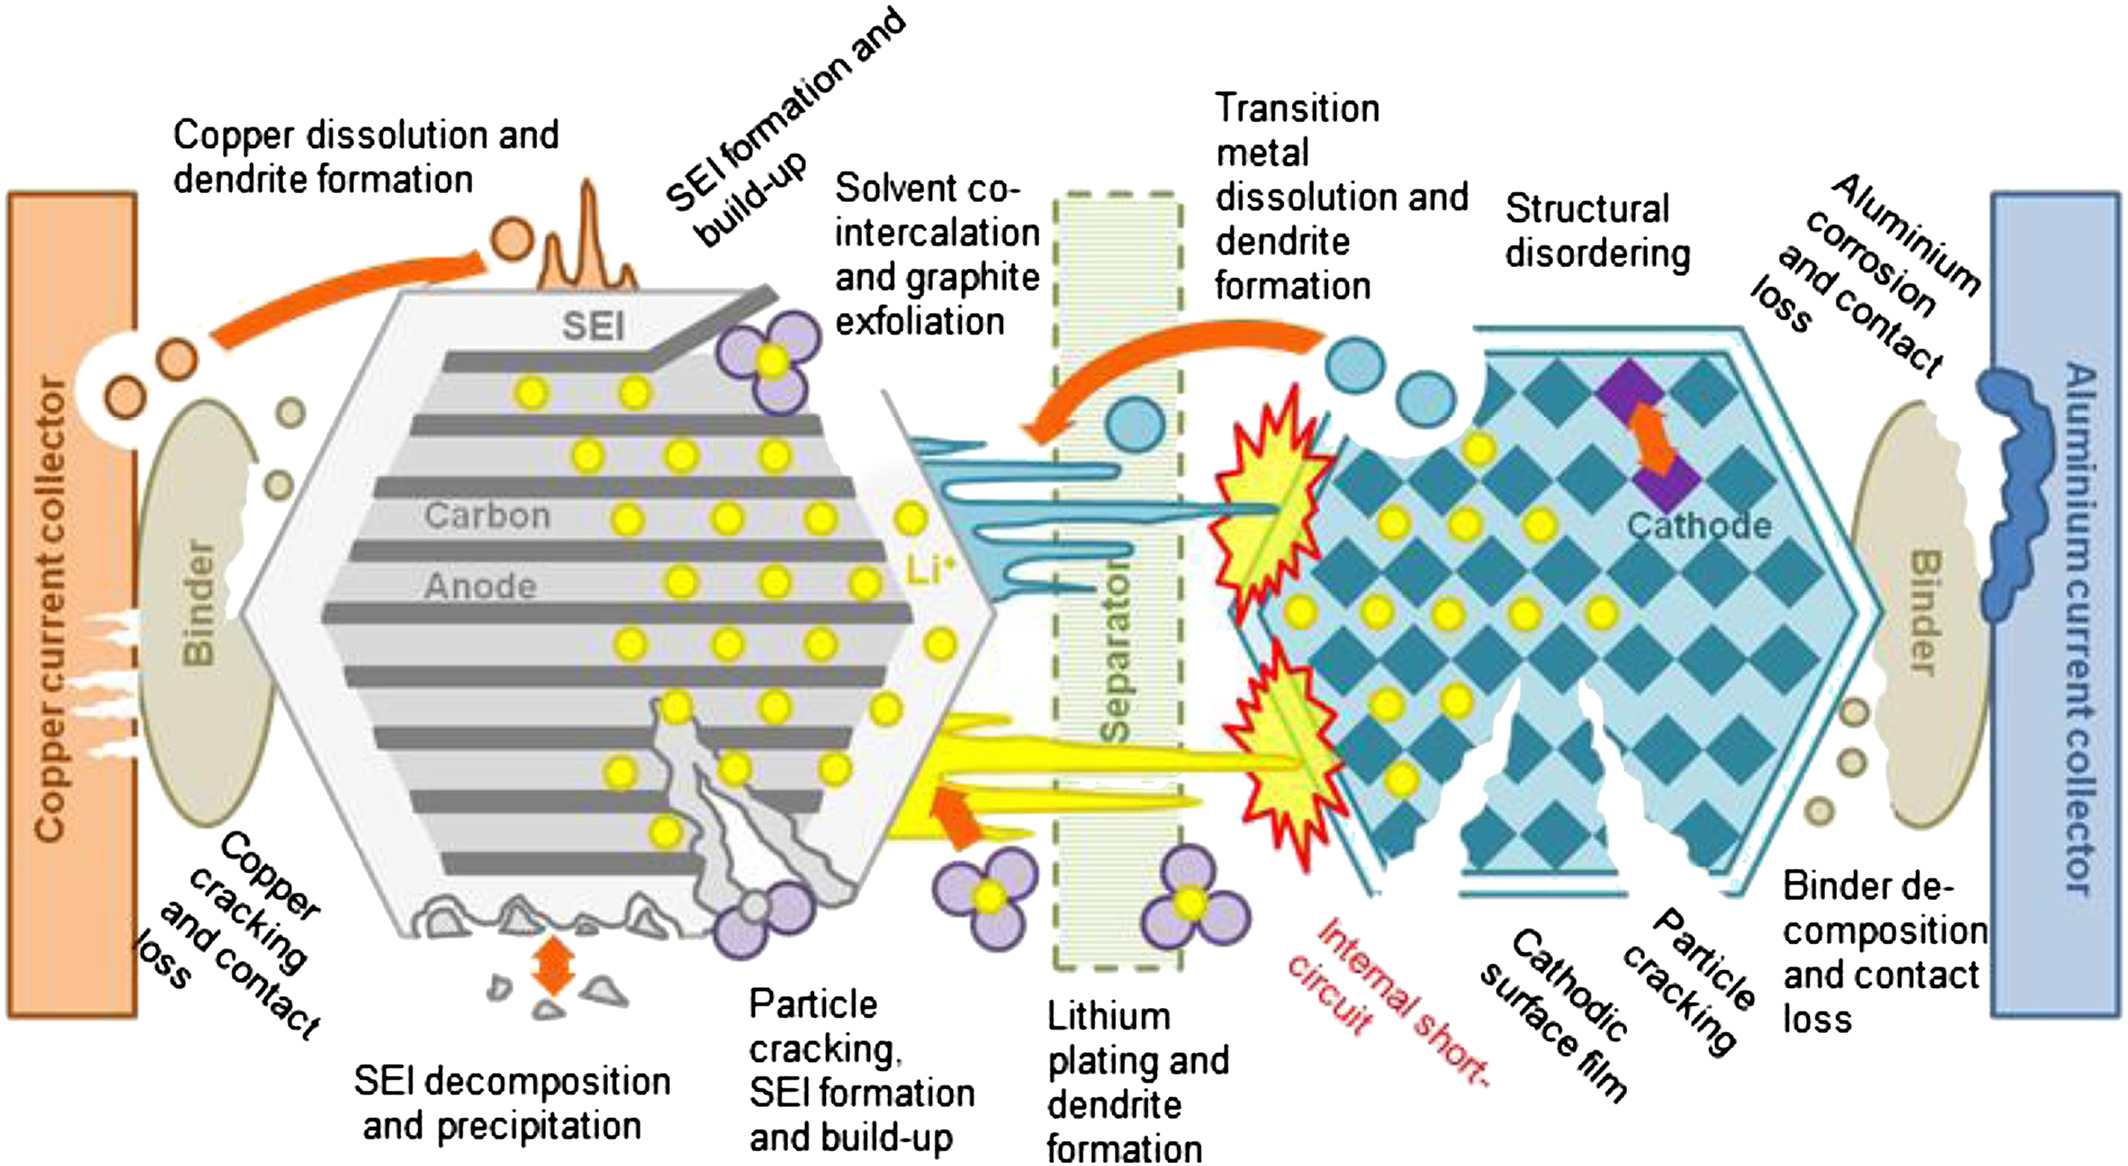
\includegraphics[width=\textwidth]{logos/Degradation mechanisms in Li-ion cells.jpg}
    \end{column}
  \end{columns}
\end{frame}

\begin{frame}{Fatores que Afetam a Degradação}
  \begin{exampleblock}{Fatores que Afetam a Degradação}
    \begin{itemize}
      \item Temperatura de operação
      \item Profundidade de descarga
      \item Taxa de carga/descarga
      \item Número de ciclos
    \end{itemize}
  \end{exampleblock}
\end{frame}

\section{Estado da Arte}
\begin{frame}{Métodos Tradicionais}
  \begin{columns}
    \begin{column}{0.48\textwidth}
      \textbf{Modelos de Circuito Equivalente}:
      \begin{itemize}
        \item Modelo de Thévenin
        \item Modelo PNGV
        \item Representam comportamento eletroquímico
      \end{itemize}
      
      \vspace{0.3cm}
      
      \textbf{Coulomb Counting}:
      \begin{itemize}
        \item Integração da corrente
        \item Acumulação de erros
        \item Limitações de precisão
      \end{itemize}
    \end{column}
    \begin{column}{0.48\textwidth}
      \textbf{Filtros de Kalman}:
      \begin{itemize}
        \item Filtro de Kalman Estendido (EKF)
        \item Estimativa de estado
        \item Fusão de sensores
      \end{itemize}
      
      \begin{alertblock}{Limitações}
        \begin{itemize}
          \item Não-linearidade
          \item Variabilidade ambiental
          \item Envelhecimento não modelado
        \end{itemize}
      \end{alertblock}
    \end{column}
  \end{columns}
\end{frame}

\begin{frame}{Métodos Baseados em IA}
  \begin{block}{Redes Neuronais Recorrentes}
    \begin{itemize}
      \item RNNs básicas com memória limitada
      \item LSTMs para dependências temporais longas
      \item Melhor modelação da degradação da bateria
    \end{itemize}
  \end{block}
  
  %\vspace{0.3cm}
  
  \begin{block}{Arquiteturas Avançadas}
    \begin{itemize}
      \item \textbf{Transformers}: Mecanismos de atenção para sequências longas
      \item \textbf{Mixture of Experts (MoE)}: Especialização para diferentes padrões
      %\item \textbf{CNNs}: Processamento de padrões espaciais/temporais
    \end{itemize}
  \end{block}
  
  \begin{exampleblock}{Vantagens da IA}
    \begin{itemize}
      \item Captura de padrões complexos e não-lineares
      \item Adaptação a diferentes condições
      \item Aprendizagem de relações ocultas
    \end{itemize}
  \end{exampleblock}
\end{frame}

\section{Desenvolvimento}
\begin{frame}{Modelação MATLAB e Simulação}
  \begin{columns}
    \begin{column}{0.5\textwidth}
      \begin{block}{Implementação EKF em Simulink}
        \begin{itemize}
          \item Framework completo de simulação
          \item Estimativa de SOC utilizando filtro de Kalman estendido
          \item Integração com modelo Batemo INR21700-p45b
        \end{itemize}
      \end{block}
    \end{column}
    
    \begin{column}{0.5\textwidth}
      \centering
      \IfFileExists{logos/batemo_blocks.png}{%
        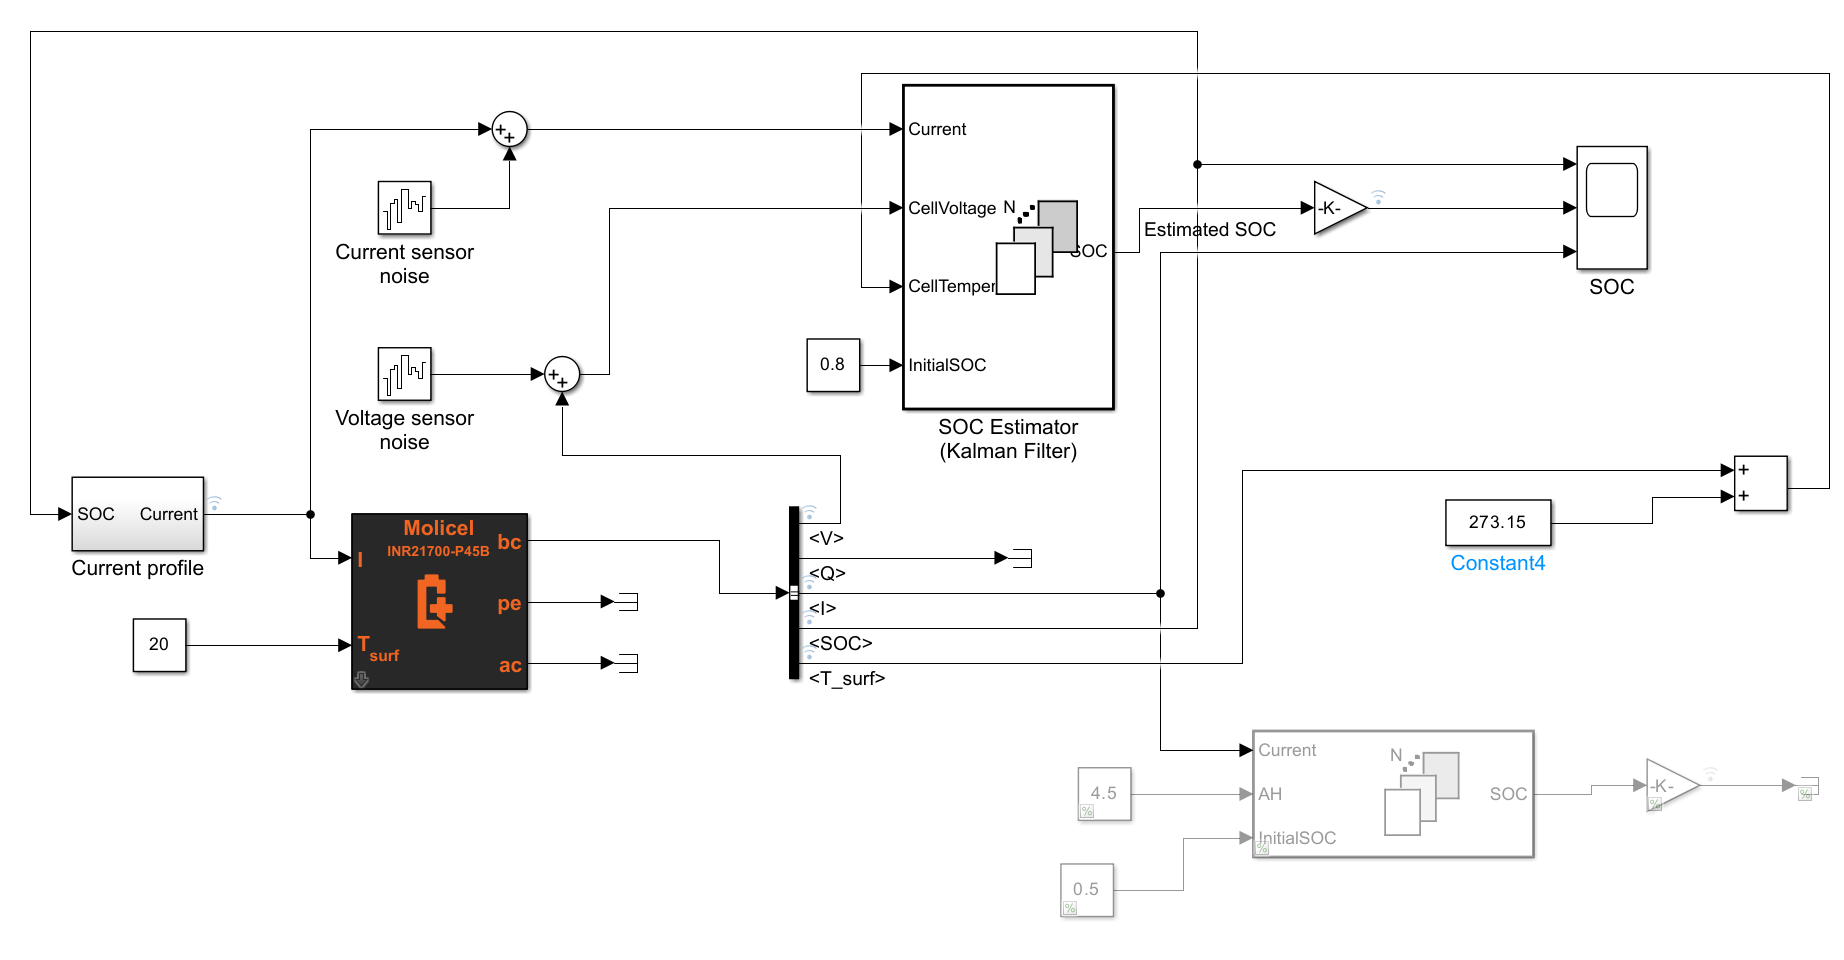
\includegraphics[width=1\textwidth]{logos/batemo_blocks.png}%
      }{%
        \fbox{\parbox{0.9\textwidth}{\centering Imagem não encontrada: logos/batemo_blocks.png}}%
      }
      \vspace{0.5cm}
      \IfFileExists{logos/EKF_results.png}{%
        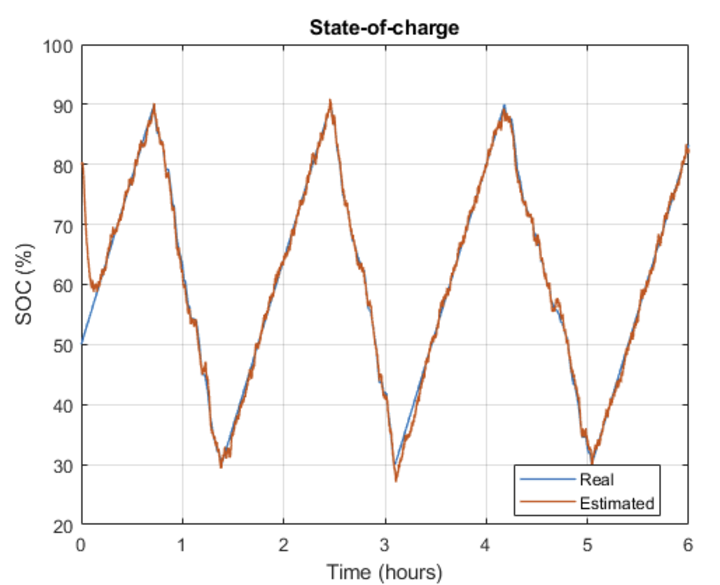
\includegraphics[width=0.7\textwidth]{logos/EKF_results.png}%
      }{%
        \fbox{\parbox{0.9\textwidth}{\centering Imagem não encontrada: logos/EKF_results.png}}%
      }
    \end{column}
  \end{columns}
\end{frame}

\begin{frame}{Arquiteturas Neuronais Baseline}
  \begin{columns}[T]
    \begin{column}{0.5\textwidth}
      \textbf{Transformer}
      \begin{itemize}
        \item Mecanismos de auto-atenção (detetar quais são os padrões mais relevantes)
        \item Excelente para sequências longas
        \item Alta precisão mas computacionalmente intensivo
      \end{itemize}
    \end{column}
    \begin{column}{0.5\textwidth}
      \centering
      \IfFileExists{logos/transformer_input.png}{%
        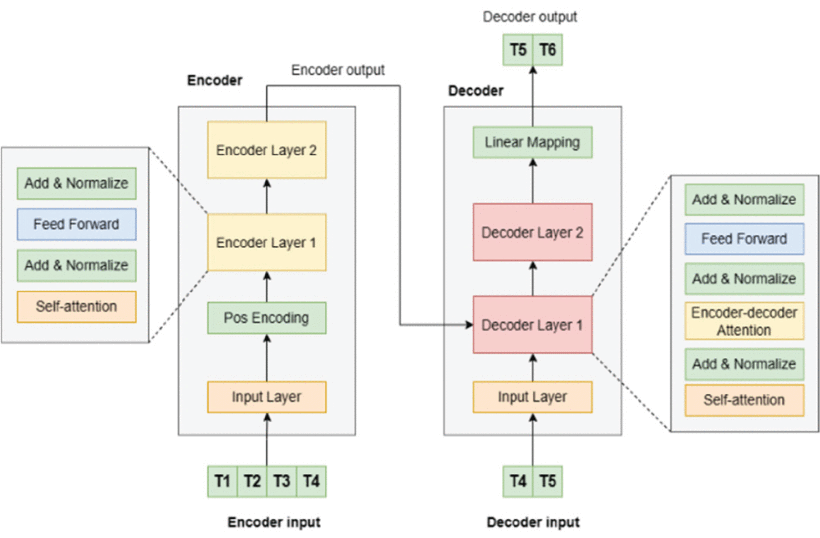
\includegraphics[width=\textwidth]{logos/transformer_input.png}%
      }{%
        \fbox{\parbox{\textwidth}{\centering Imagem não encontrada: logos/transformer_input.png}}%
      }
    \end{column}
  \end{columns}
\end{frame}

\begin{frame}{Arquiteturas Neuronais Baseline: Mixture of Experts}
  \begin{columns}[T]
    \begin{column}{0.5\textwidth}
      \textbf{Mixture of Experts}
      \begin{itemize}
        \item Rede de roteamento com especialistas
        \item Eficiente -- ativa apenas especialistas relevantes
        \item Adequado para multi-tarefas
      \end{itemize}
    \end{column}
    \begin{column}{0.5\textwidth}
      \centering
      \IfFileExists{logos/Moe_arq.png}{%
        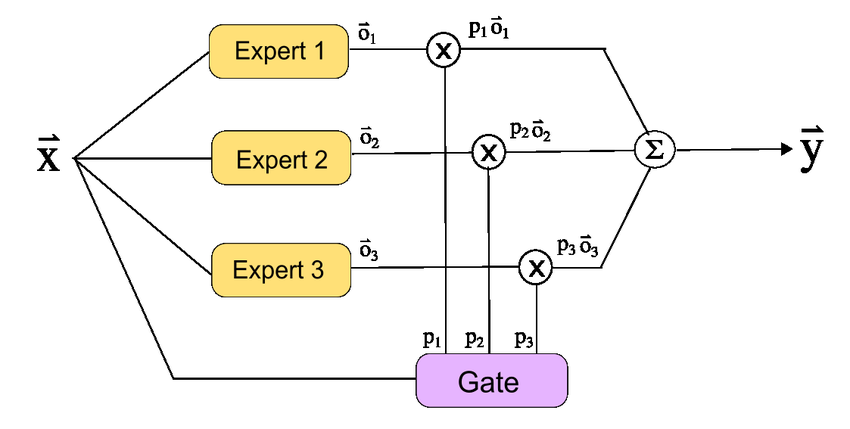
\includegraphics[width=0.8\textwidth]{logos/Moe_arq.png}%
      }{%
        \fbox{\parbox{0.8\textwidth}{\centering Imagem não encontrada: logos/Moe_arq.png}}%
      }
    \end{column}
  \end{columns}
\end{frame}

\begin{frame}{Comparação de Desempenho: Dataset CALCE CS2}
  \begin{table}
    \centering
    \caption{Comparação de Desempenho na Previsão de RUL, Raiz do Erro Quadrático Médio}
    \begin{tabular}{lc}
      \toprule
      \textbf{Modelo} & \textbf{RMSE} \\
      \midrule
      Transformer & \textbf{0.0297} \\ 
      FCN MoE & 0.0335 \\
      \bottomrule
    \end{tabular}
  \end{table}
\end{frame}

\begin{frame}{Visualização dos Resultados de Previsão de RUL}
  \begin{figure}
    \centering
    \begin{minipage}{0.45\textwidth}
      \centering
      \IfFileExists{logos/transf_graph_results.png}{%
        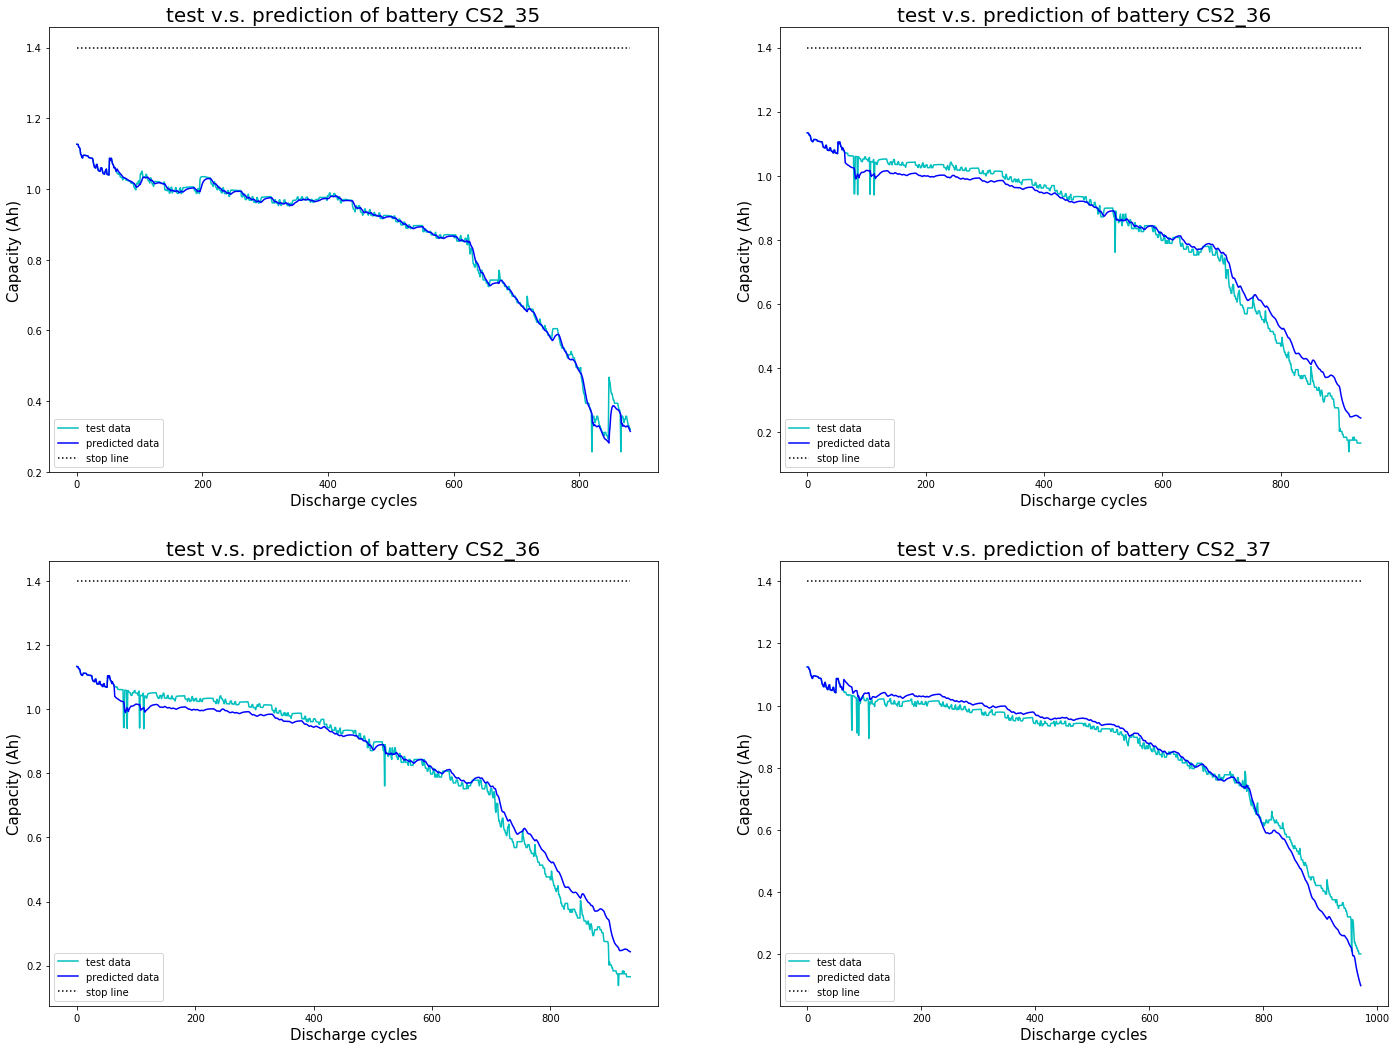
\includegraphics[width=\textwidth]{logos/transf_graph_results.png}%
        \caption{Resultados do Transformer}
      }{%
        \fbox{\parbox{\textwidth}{\centering Imagem não encontrada: logos/transf_graph_results.png}}%
      }
    \end{minipage}
    \hfill
    \begin{minipage}{0.45\textwidth}
      \centering
      \IfFileExists{logos/moe_graph_results.png}{%
        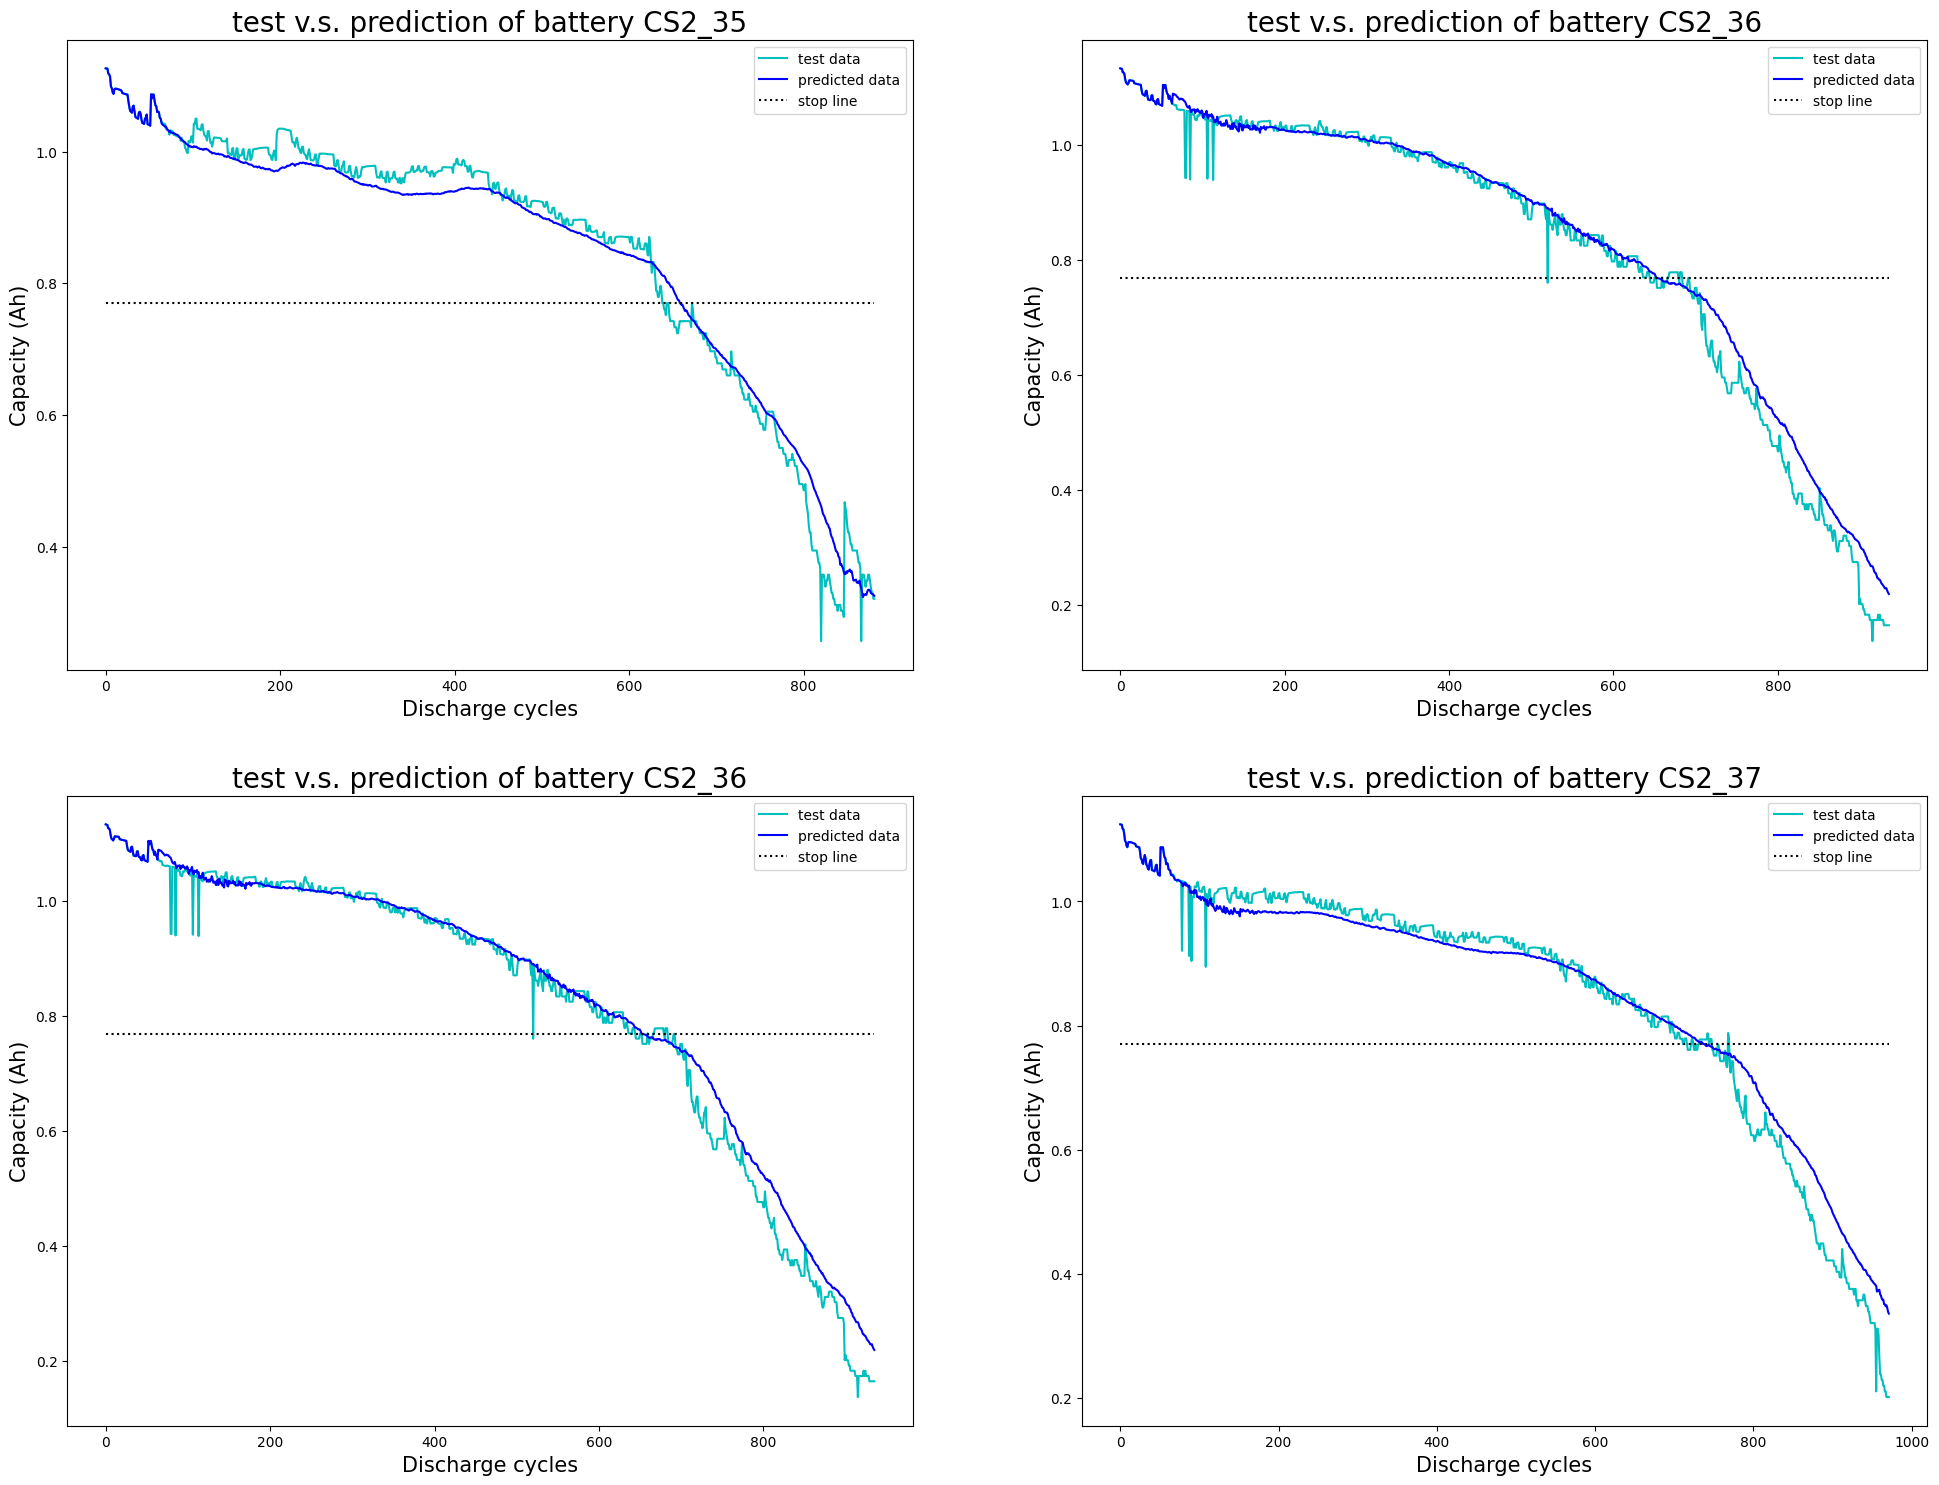
\includegraphics[width=\textwidth]{logos/moe_graph_results.png}%
        \caption{Resultados do MoE}
      }{%
        \fbox{\parbox{\textwidth}{\centering Imagem não encontrada: logos/moe_graph_results.png}}%
      }
    \end{minipage}
  \end{figure}
\end{frame}

\begin{frame}{Método Escolhido: TimesNet}
  \begin{block}{Porquê TimesNet?}
    \begin{itemize}
      \item \textbf{Especialização}: Concebido especificamente para análise de séries temporais
      \item \textbf{Multi-periodicidade}: Deteta múltiplos padrões temporais simultaneamente
      \item \textbf{Transformação 2D}: Converte dados 1D em tensors 2D para processamento com CNNs
    \end{itemize}
  \end{block}
  
  \vspace{0.3cm}
  
  \centering
  \IfFileExists{logos/timesnet_2d_structure.pdf}{%
    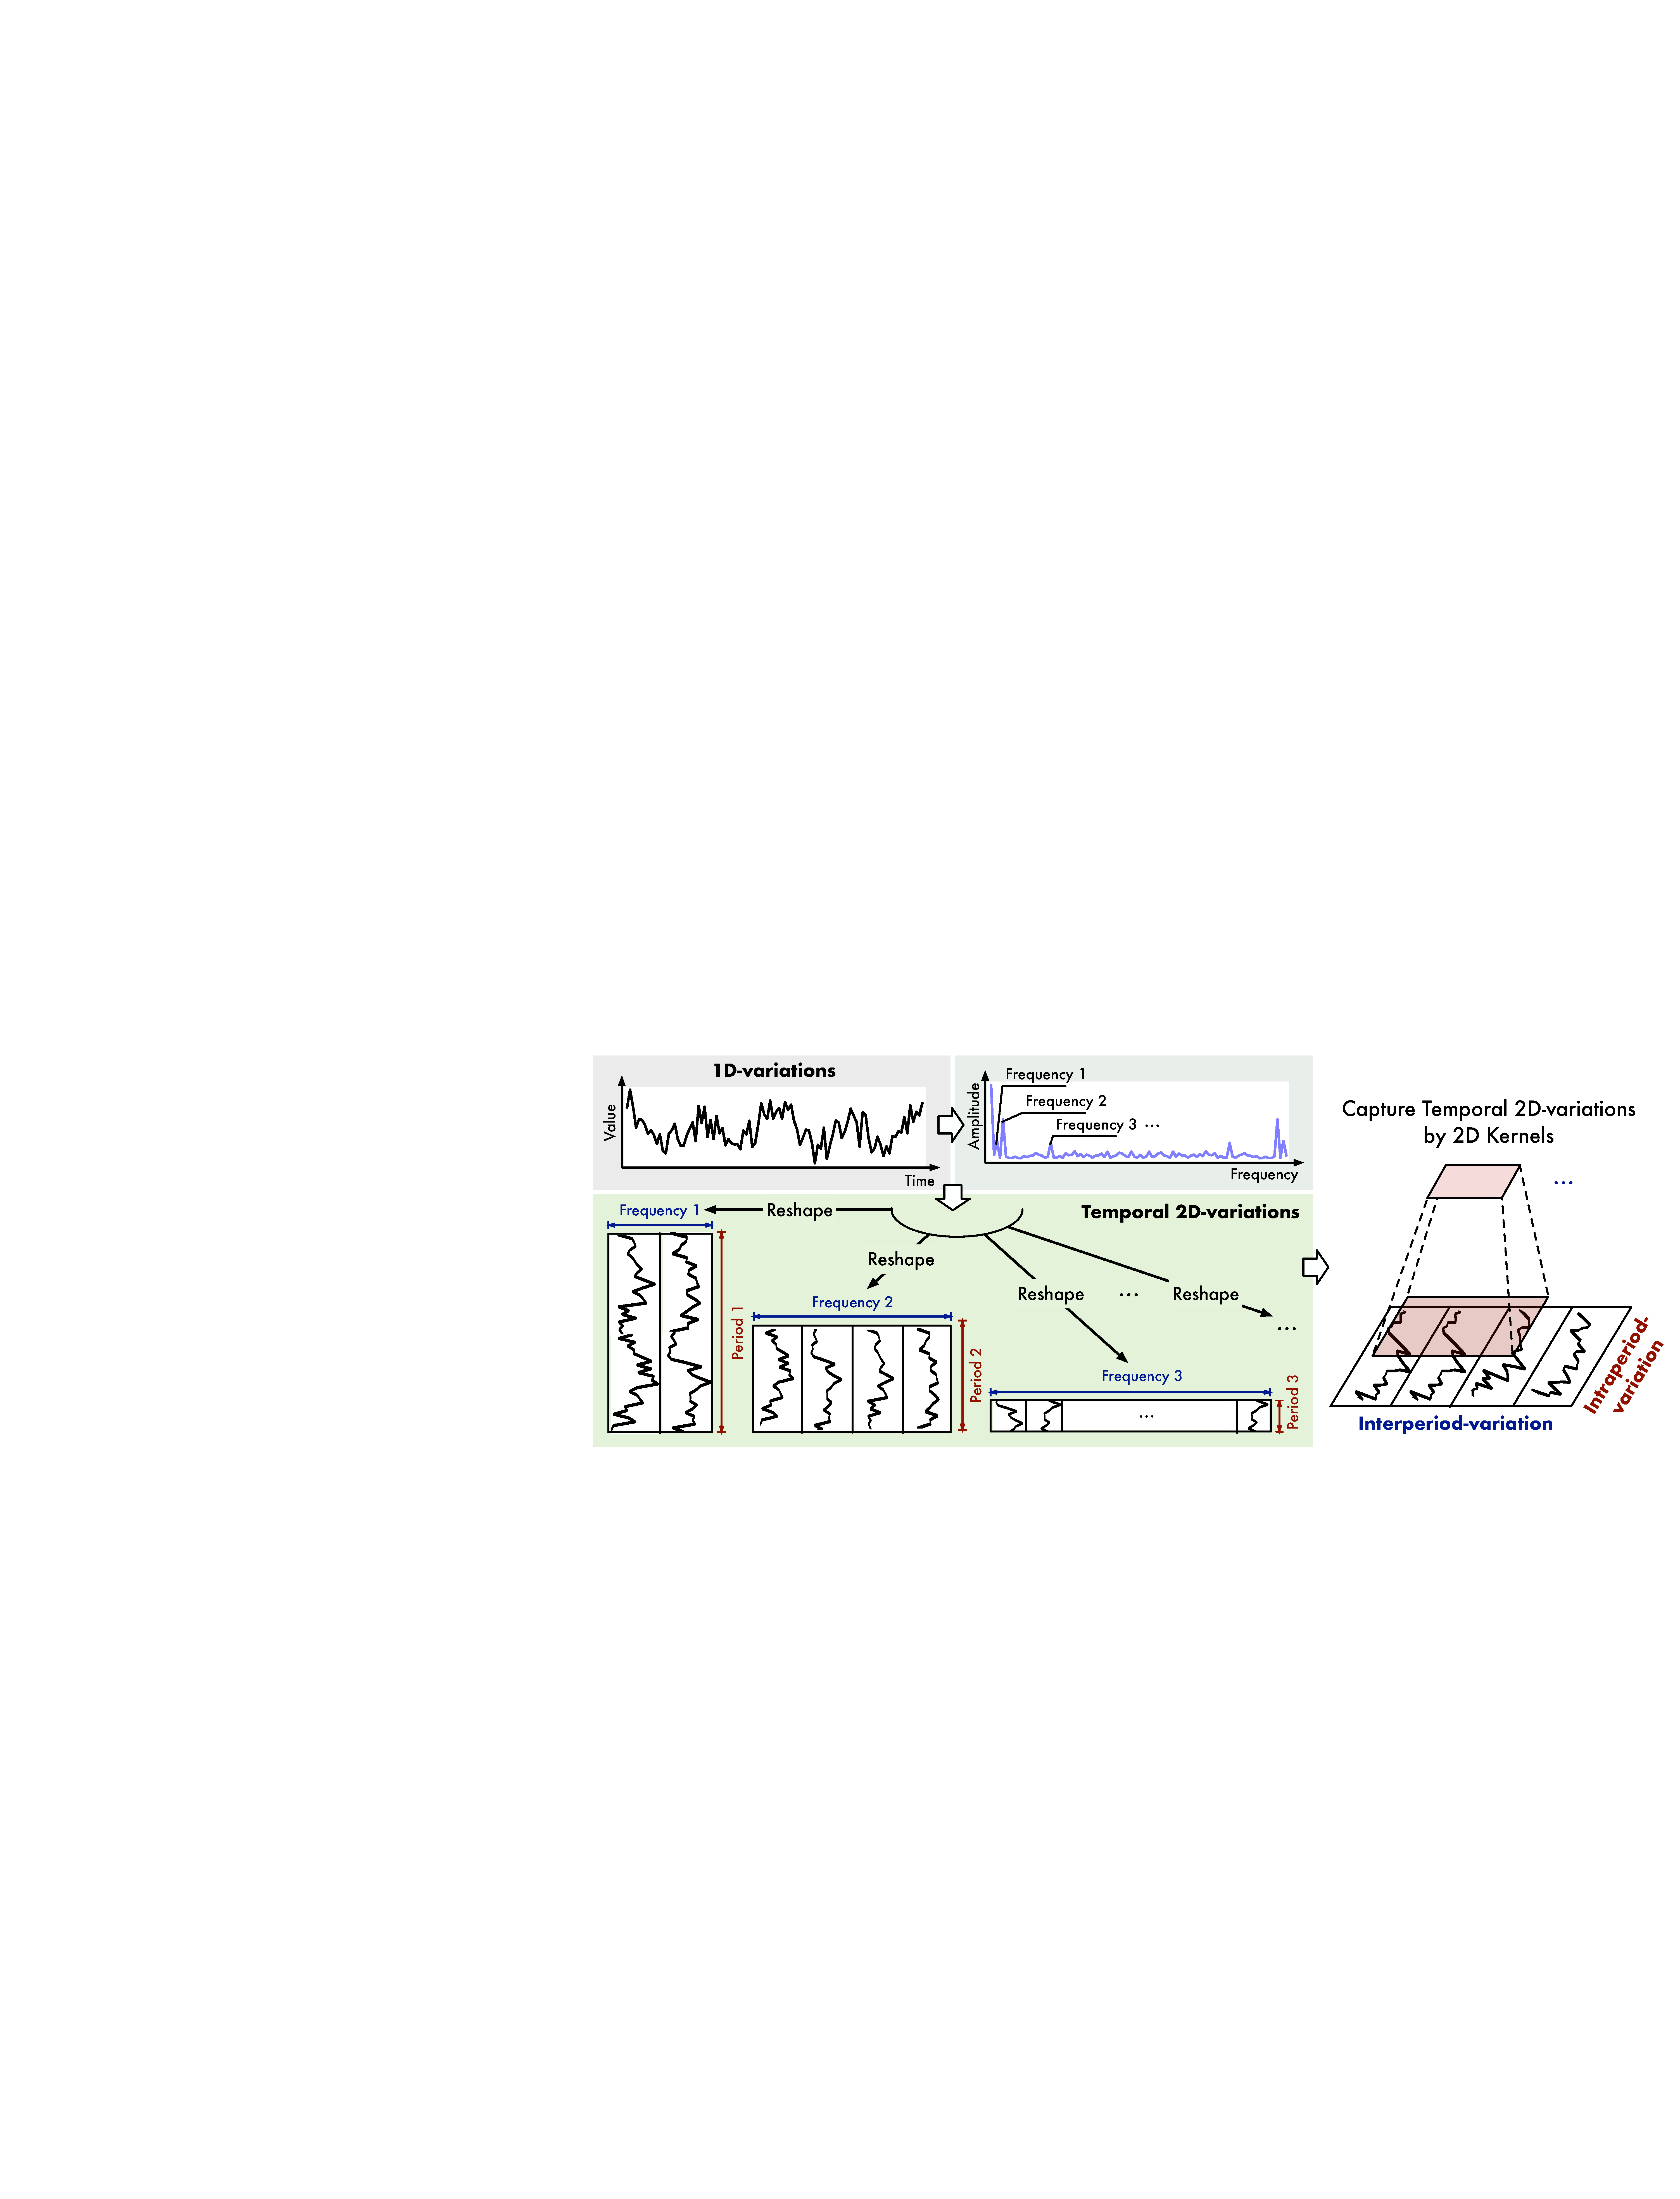
\includegraphics[width=0.8\textwidth]{logos/timesnet_2d_structure.pdf}%
  }{%
    \fbox{\parbox{0.8\textwidth}{\centering Imagem não encontrada: logos/timesnet_2d_structure.pdf}}%
  }
\end{frame}

\begin{frame}{Método Escolhido: TimesNet}
  \begin{exampleblock}{Vantagens para Dados de Bateria}
    \begin{itemize}
      \item Captura padrões de curto prazo (ciclos de carga/descarga)
      \item Deteta tendências de longo prazo (degradação)
      \item Usa FFTs para facilitar a descoberta de periodicidades
    \end{itemize}
  \end{exampleblock}
\end{frame}

\begin{frame}{Dataset CALCE CS2}
  \begin{block}{Características do Dataset}
    \begin{itemize}
      \item \textbf{~880 ciclos} de operação por cada bateria Li-ion do dataset CALCE CS2
      \item Medições incluem tensão, corrente, tempo, temperatura, capacidade, etc.
      \item Dados organizados sistematicamente por multiplos ciclos de carga/descarga
    \end{itemize}
  \end{block}
    \begin{figure}
    \centering
    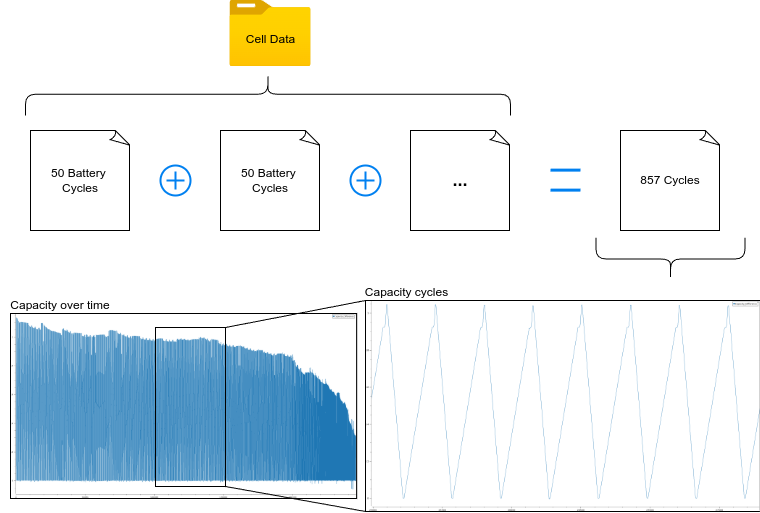
\includegraphics[width=0.5\textwidth]{logos/cycles_files.png}
    \caption{Visualização dos ciclos de operação do dataset CALCE CS2}
  \end{figure}
\end{frame}

\begin{frame}{Metodologia de Pré-processamento}

  \begin{exampleblock}{Metodologia de Pré-processamento}
    \begin{itemize}
      \item Cálculo derivado de SOC, SOH e RUL com base nos dados de capacidade
      \item Segmentação em ciclos
      \item Divisão do dataset: 70\% treino, 15\% validação, 15\% teste
    \end{itemize}
  \end{exampleblock}
  
  \vspace{0.3cm}
  
  \begin{block}{Adaptação}
    \begin{itemize}
      \item \textbf{Entradas}: Tensão, corrente, tempo.
      \item \textbf{Alvos}: SOC, SOH, RUL
    \end{itemize}
  \end{block}
\end{frame}

\begin{frame}{Metodologia e Otimização de Hiperparâmetros}
  \begin{columns}[T] % Aligns the top of the columns
    % --- Left Column ---
    \column{0.5\textwidth}
      \begin{block}{Ferramentas e Processo}
        \begin{itemize}
          \item \textbf{Ferramentas:}
            \begin{itemize}
              \item Optuna para otimização
              \item Weights \& Biases para monitorização
            \end{itemize}
          \item \textbf{Processo:}
            \begin{itemize}
              \item 50 tentativas, cada uma com 50 epochs
              \item Objetivo: Minimizar o MSE na validação
            \end{itemize}
        \end{itemize}
      \end{block}

    % --- Right Column ---
    \column{0.5\textwidth}
      \begin{exampleblock}{Parâmetros Otimizados}
        \begin{itemize}
          \item \texttt{e\_layers}: Nº de camadas do encoder (1-3)
          \item \texttt{d\_layers}: Nº de camadas do decoder (1-3)
          \item \texttt{factor}: Fator de expansão para a FFN (1-5)
          \item \texttt{freq}: Frequência para codificação temporal
          \item \texttt{top\_k}: Nº de frequências dominantes (TimesNet)
        \end{itemize}
      \end{exampleblock}
  \end{columns}
\end{frame}

\begin{frame}{Visualização da Otimização}
  \begin{columns}
    \column{0.5\textwidth}
      \centering
      \begin{figure}
        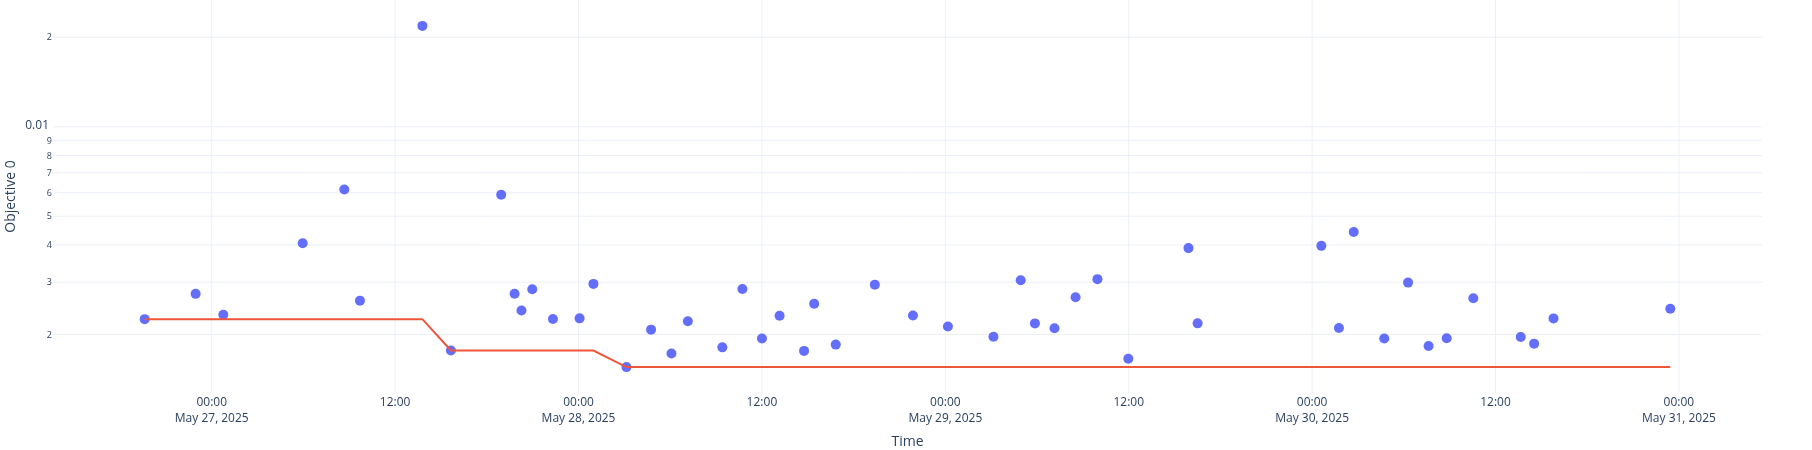
\includegraphics[width=1\textwidth]{logos/optuna_objective_plot.png}
        \caption{Optuna Objective Plot}
      \end{figure}
    \column{0.5\textwidth}
      \centering
      \begin{figure}
        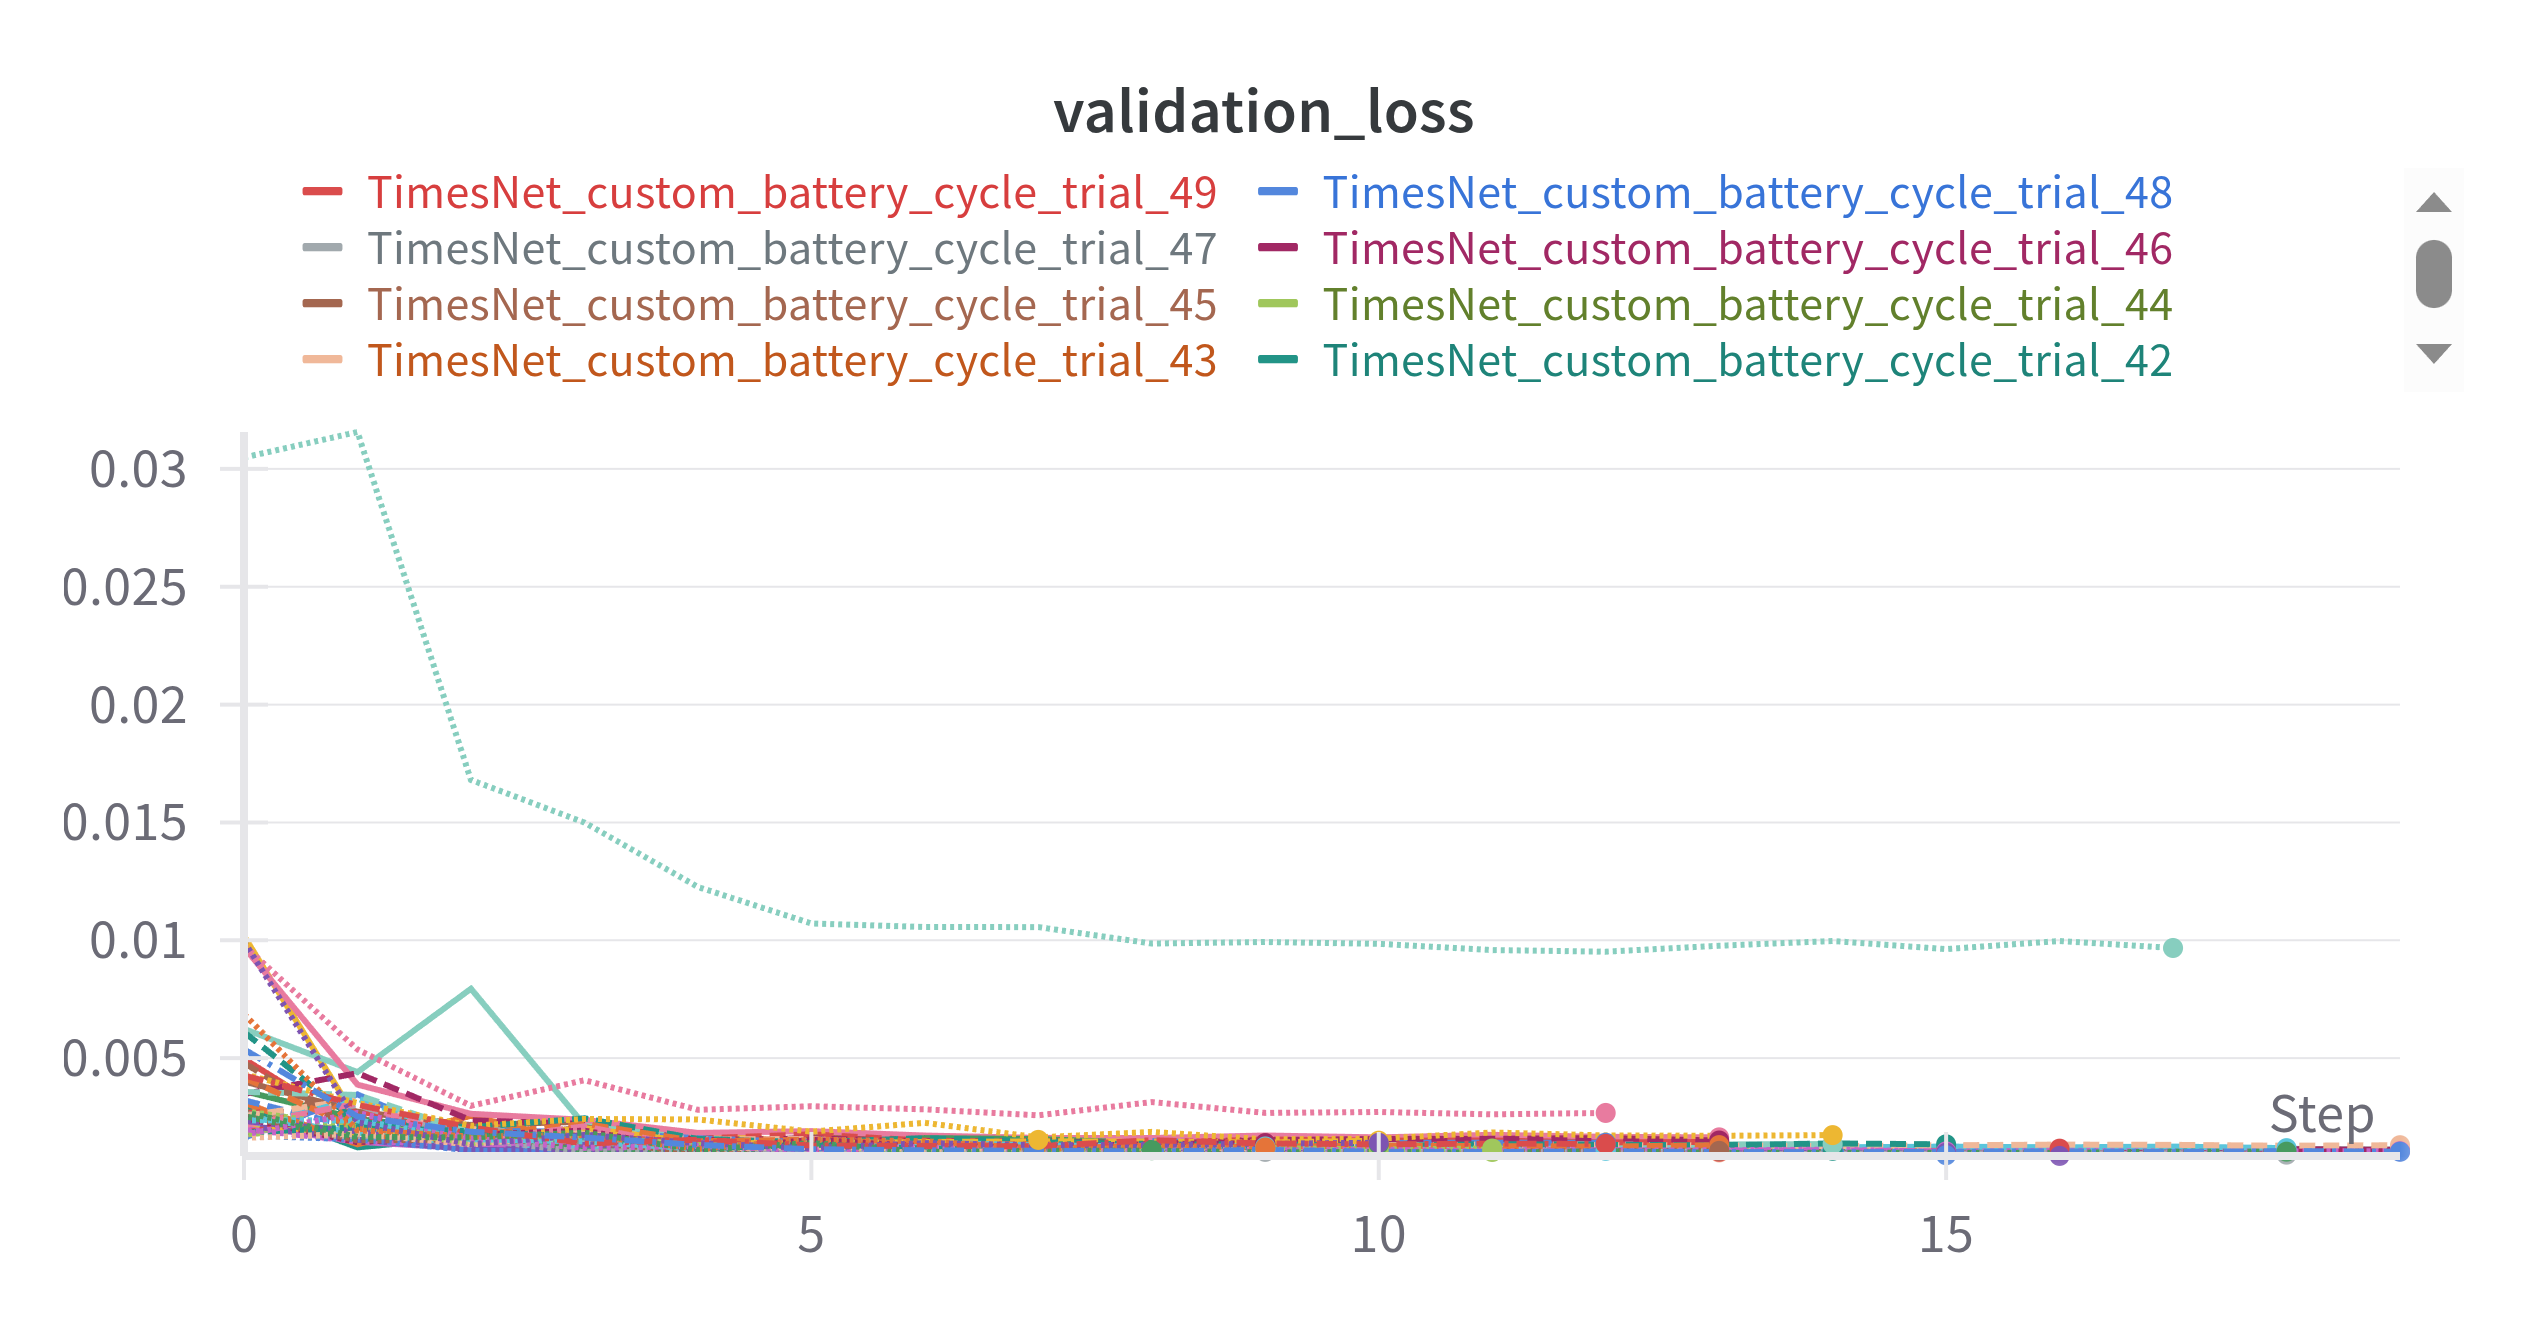
\includegraphics[width=1\textwidth]{logos/W&B_optimization_validation_loss.png}
        \caption{W\&B Validation Loss}
      \end{figure}
  \end{columns}
\end{frame}

\section{Experiências e Resultados}
\begin{frame}{Configuração e Desempenho do Modelo}
  \begin{columns}[T]
    \begin{column}{0.48\textwidth}
      \begin{block}{Configuração Final}
        \begin{itemize}
          \item \textbf{43 Epochs} de treino
          \item Loss de validação final: \textbf{0,02939}
          \item Arquitetura com \textbf{37,5M parâmetros}
          \item Memória ocupada: 140 MB
        \end{itemize}
      \end{block}
      
      \vspace{0.3cm}
      
      \begin{exampleblock}{Divisão dos Dados}
        \begin{itemize}
          \item ~120000 amostras para treino (70\%)
          \item ~4900 amostras para validação (15\%)
          \item ~4900 amostras para teste (15\%)
        \end{itemize}
      \end{exampleblock}
    \end{column}
    \begin{column}{0.48\textwidth}
      \begin{table}
        \centering
        \caption{Métricas de Desempenho por Parâmetro}
                  \resizebox{0.6\textwidth}{!}{%
        \begin{tabular}{lcc}
          \toprule
          \textbf{Parâmetro} & \textbf{RMSE} & \textbf{MAE} \\
          \midrule
          SOC & \textbf{0,2251} & \textbf{0,0621} \\
          SOH & 0,5282 & 0,2039 \\
          RUL & 0,5311 & 0,2078 \\
          \bottomrule
        \end{tabular}
        }
      \end{table}
    
      
      \centering
      \begin{figure}
        \centering
        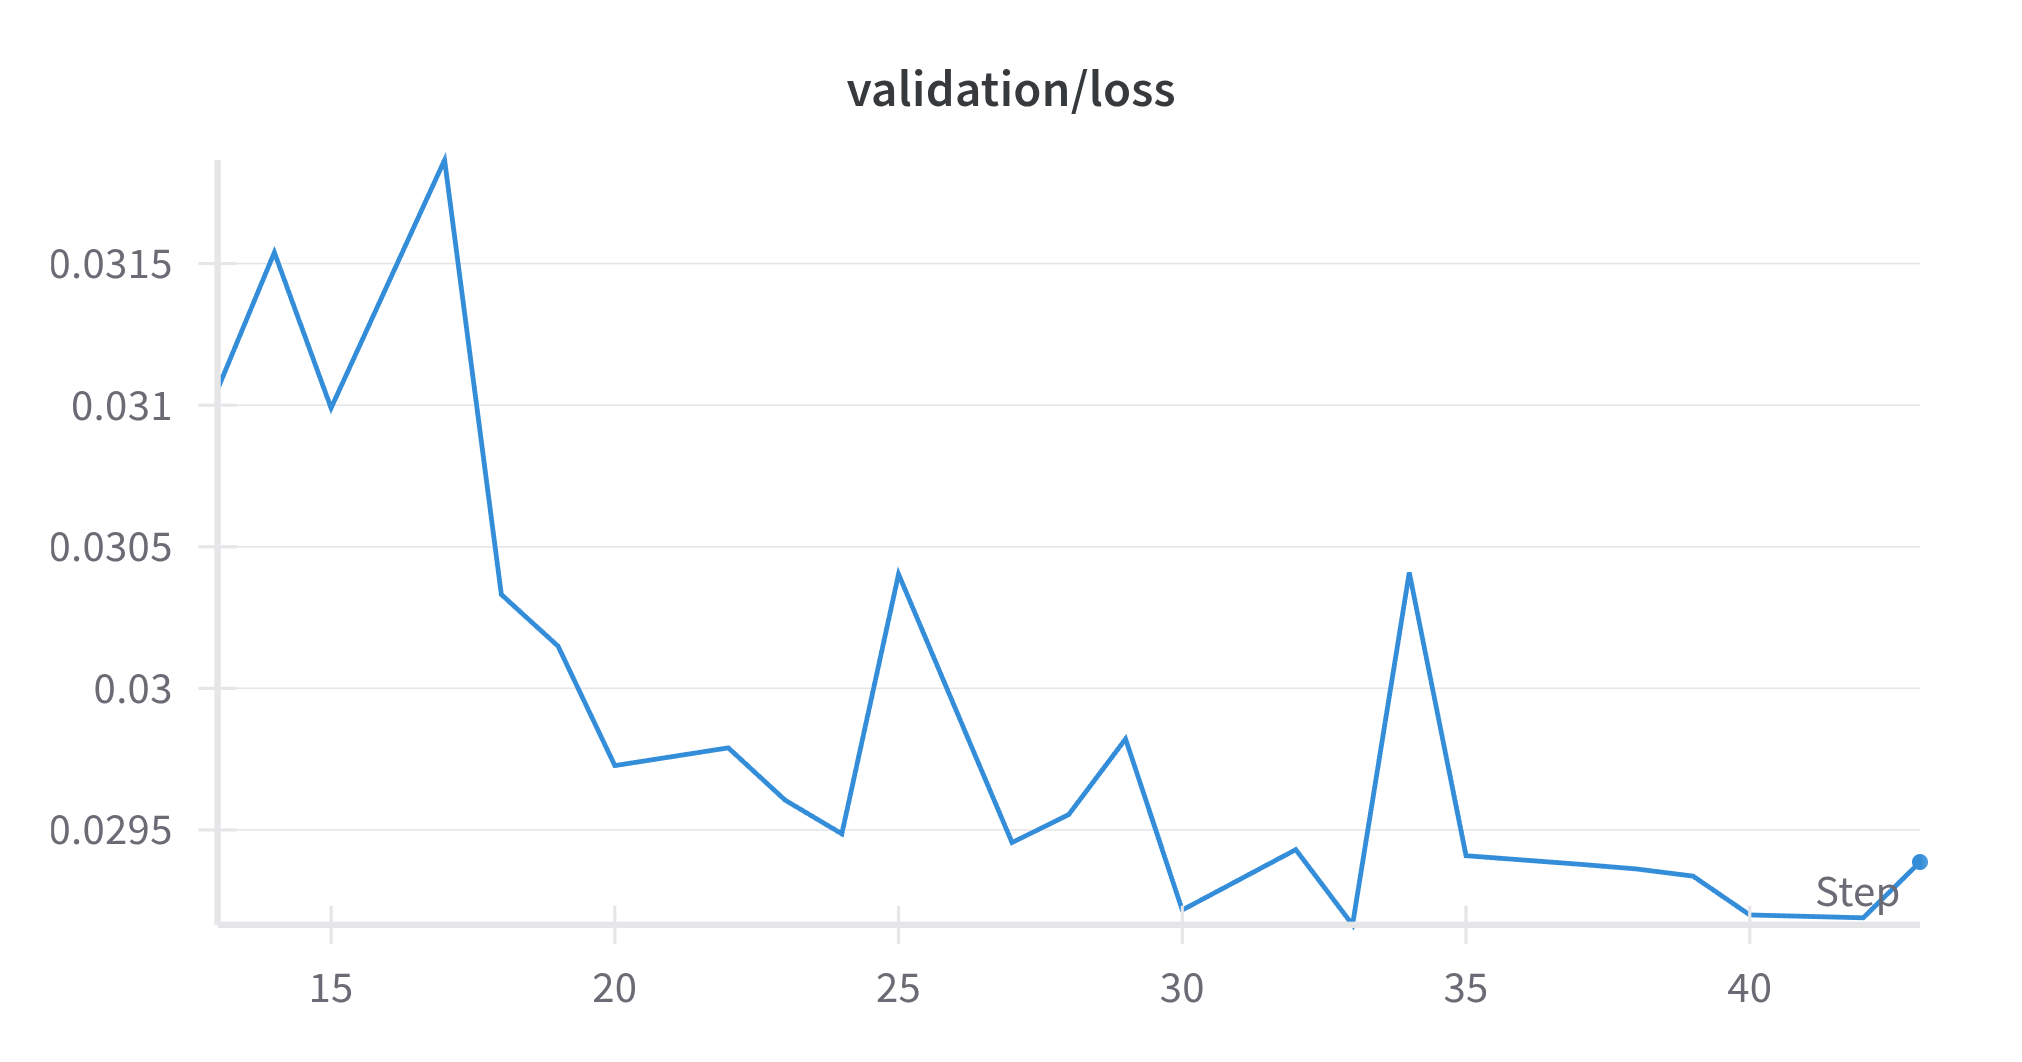
\includegraphics[width=\textwidth]{logos/validation_loss.png}
        \caption{Curva de perda de validação durante o treinamento}
      \end{figure}
    \end{column}
  \end{columns}
\end{frame}

\begin{frame}{Análise de Resultados e Hierarquia de Desempenho}
  \begin{columns}[T]
    \begin{column}{0.48\textwidth}
      \begin{exampleblock}{Desempenho}
        \begin{enumerate}
          \item \textbf{SOC}: Melhor precisão (RMSE: 0,2251)
            \begin{itemize}
              \item Correlação direta com medições elétricas
              \item Padrões cíclicos bem definidos
            \end{itemize}
          \item \textbf{SOH}: Desempenho moderado (RMSE: 0,5282)
            \begin{itemize}
              \item Degradação gradual mais complexa
            \end{itemize}
          \item \textbf{RUL}: Maior desafio (RMSE: 0,5311)
            \begin{itemize}
              \item Previsão de tendências futuras
            \end{itemize}
        \end{enumerate}
      \end{exampleblock}
    \end{column}
    \begin{column}{0.48\textwidth}
      \begin{figure}
        \centering
        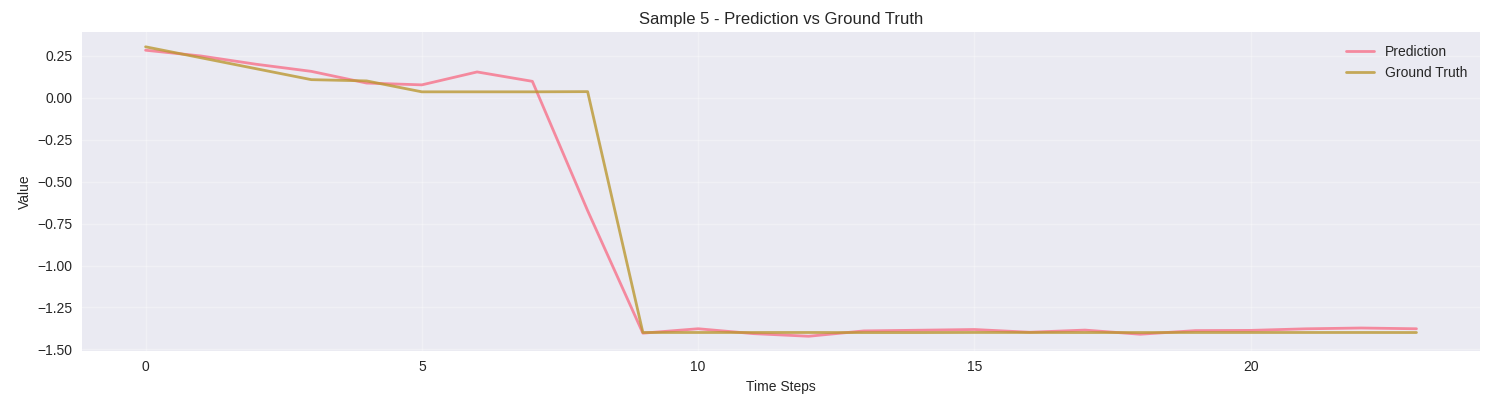
\includegraphics[width=\textwidth]{logos/soc_prediction2.png}
        \caption{Valores reais vs preditos (SOC)}
      \end{figure}
        \begin{table}[h]
          \centering
          \caption{Comparação de Abordagens (RMSE em RUL)}
          \resizebox{0.6\textwidth}{!}{%
          \begin{tabular}{lc}
            \toprule
            \textbf{Modelo} & \textbf{RMSE} \\
            \midrule
            Transformer (tarefa única) & 0,0297 \\
            MoE (tarefa única) & 0,0335 \\
            TimesNet (multi-tarefa) & 0,5311 \\
            \bottomrule
          \end{tabular}%
          }
        \end{table}
        \centering
        \small{(Utilizando o mesmo dataset CALCE CS2)}

    \end{column}
  \end{columns}
\end{frame}

\begin{frame}{Desafios da Abordagem Multi-tarefa}
  \begin{columns}[T]
    \begin{column}{0.48\textwidth}
      \begin{block}{Principais Limitações}
        \begin{itemize}
          \item \textbf{Temporais}: SOC (curto prazo) vs SOH/RUL (longo prazo)
          \item \textbf{Computacionais}: 37,5M parâmetros (140 MB)
          \item \textbf{Treino}: Gradientes em conflito entre tarefas
          \item \textbf{Implementação}: Inviável em sistemas embebidos
        \end{itemize}
      \end{block}
    \end{column}
    \begin{column}{0.48\textwidth}
      \begin{exampleblock}{Impacto no Desempenho}
        \begin{itemize}
          \item Neste caso o modelo especializado supera a abordagem unificada
          \item 18x pior no RMSE para RUL (0,0297 → 0,5311)
        \end{itemize}
      \end{exampleblock}
      
      \vspace{0.3cm}
      
      \begin{alertblock}{Conclusão}
        \centering
        Soluções abrangentes nem sempre são ótimas para problemas específicos como monitorização de baterias.
      \end{alertblock}
    \end{column}
  \end{columns}
\end{frame}

\section{Discussão e Análise}

\begin{frame}{Limitações e Direções Futuras}
  \begin{columns}[T]
    \begin{column}{0.48\textwidth}
      \begin{alertblock}{Limitações do Estudo}
        \begin{itemize}
          \item \textbf{Generalização limitada}: Dataset CALCE CS2
          \item \textbf{Gap laboratorial}: Condições controladas vs. reais
          \item \textbf{Diversidade química}: Li-ion específicas
          \item \textbf{Implementação}: Elevados requisitos computacionais
        \end{itemize}
      \end{alertblock}
      
      \vspace{0.2cm}
      
      
    \end{column}
    \begin{column}{0.48\textwidth}
      \begin{exampleblock}{Direções Futuras}
        \begin{itemize}
          \item \textbf{Ensemble methods}: CNNs para SOC, LSTMs para RUL
          \item \textbf{Transfer learning}: Reutilizar conhecimento entre tipos de baterias
          \item \textbf{Model compression}: Distilação, pruning e quantização
        \end{itemize}
      \end{exampleblock}
    \end{column}
  \end{columns}
  \begin{block}{Lição Principal}
        \small
        Resolver SOC, SOH e RUL simultaneamente pode não ser ideal para desempenho superior individual.
      \end{block}
\end{frame}

\begin{frame}[plain]
  \centering
  \Huge \textbf{Obrigado!}
  
  \vspace{1cm}
  
  \Large \textbf{BattAIHealth}
  
  \normalsize
  \textbf{Battery Condition Estimation in Automotive and Railway Applications Using AI}
  
  \vspace{1cm}
  
  \normalsize
  Perguntas e Discussão
  
  \vspace{0.5cm}
  \small
  Pedro André Silva Ferreira
  Projeto Final - Engenharia Eletrotécnica e de Computadores
  Instituto Politécnico de Leiria
  Julho 2025
\end{frame}

\begin{frame}{Referências Principais}
  \begin{thebibliography}{9}
    \small
    \bibitem{timesnet}
      Haixu Wu, Tengge Hu, Yong Liu, Hang Zhou, Jianmin Wang, Mingsheng Long.
      \emph{TimesNet: Temporal 2D-Variation Modeling for General Time Series Analysis}.
      arXiv:2210.02186 [cs], 2023. doi: 10.48550/arXiv.2210.02186.
    
    \bibitem{calce}
      CALCE Battery Research Group.
      \emph{Battery Data | Center for Advanced Life Cycle Engineering}.
      University of Maryland. \url{https://calce.umd.edu/battery-data}
      
    \bibitem{chen2022}
      Daoquan Chen, Weicong Hong, Xiuze Zhou.
      \emph{Transformer Network for Remaining Useful Life Prediction of Lithium-Ion Batteries}.
      IEEE Access, vol. 10, pp. 19621--19628, 2022. doi: 10.1109/ACCESS.2022.3151975.
      
    \bibitem{optuna}
      Takuya Akiba, Shotaro Sano, et al.
      \emph{Optuna: A Next-generation Hyperparameter Optimization Framework}.
      KDD, 2019.
      
    \bibitem{moe}
      Noam Shazeer, Azalia Mirhoseini, et al.
      \emph{Outrageously Large Neural Networks: The Sparsely-Gated Mixture-of-Experts Layer}.
      ICLR, 2017.
  \end{thebibliography}
\end{frame}

\end{document}